%%body for test 1

\ques{15}
Consider the following {\bf MINIMIZING}, canonical form linear program, labeled (P):
\vspace{-2mm}

\begin{equation}
  \label{eq:1}
  \tag{P}
  \begin{array}{lll}
    \min & 2 x_1 \phantom{+ x_2} - 3 x_3 + 18 x_4 & \\
    \mbox{s.t.} & x_1 -  x_2 + 2 x_3 + x_4 & = 4 \\[1mm]
    & x_1 + x_2 \phantom{+ x_3} + 3 x_4 & = 2 \\
    & x_1, x_2, x_3, x_4 \geq 0 &
  \end{array}
\end{equation}



\begin{parts}
\pts{6} Assume that $x_1$ and $x_3$ are basic.  Solve for the current basic feasible solution.


\vspace{1cm}

Because $x_2$ and $x_4$ are nonbasic we have $x_2 = 0$ and $x_4 = 0$.  Then, by inspection of the second constraint, $x_1 = 2$.  It then follows from the first constraint that $x_3 = 1$.

\vfill


\pts{3} Given the feasible direction $d^{x_2} = [-1, 1, 1, 0]^T$ associated with the basis $\mathcal{B} = \{x_1, x_3\}$, determine whether or not it is an improving direction.  Based on your answer about whether the direction is improving, state whether the simplex algorithm would continue or terminate at this point.  {\bf Briefly} explain your answer for full credit.  You may find it helpful to recall that $\bar c_k = c^T d^k = c_k + \sum_{i \in \mathcal{B}} c_i d_i^k$.

We calculate the reduced cost for the nonbasic variable $x_2$ as follows: $\bar c_{x_2} = [2, 0, -3, 18]   \begin{bmatrix}
    -1 \\ 1 \\ 1 \\ 0
  \end{bmatrix} = -2 - 3 = -5$.  Because we have a minimization problem and the reduced cost is negative, this is an improving simplex direction.  This means our current solution is not optimal, and the simplex algorithm will continue.

\vfill

\pts{3} For the simplex direction $d^{x_2} = [-1, 1, 1, 0]^T$ associated with the basis $\mathcal{B} = \{x_1, x_3\}$, use the ratio test to find the maximum step size, $\lambda$.  Based on your answer about $\lambda$, which variable will leave the basis and become nonbasic?    You may find it helpful to recall that 

\[
\lambda_{max} = \min \left\{ \frac{x_j}{-d_j^k}:d_j^k < 0 \right\}
\]

\vspace{0.5cm}
The improving simplex direction has one negative component, so we apply the rule given above to find $\lambda_{max} = \frac{2}{1} = 2$.  Because $x_1$ defines the maximum step size, it will leave the basis and become nonbasic.  
\vspace{0.5cm}

\pts{3} Use your answers from parts a and c above to compute the new solution generated by this iteration of the Simplex Method. 

\[
x_{\text{new}} = x_\text{old} + \lambda_{max} d = [2,0,1,0]^T + 2 [-1,1,1,0]^T = [0,2,3,0]^T
\]



\end{parts}

\newpage

%%formulation given to answer about
\ques{20} Consider the directed network shown below, where the numbers on the arcs represent cost, $c_{ij}$, to send one unit of flow along the arc.  Use the start of a formulation given below to answer the following questions.

\begin{center}
        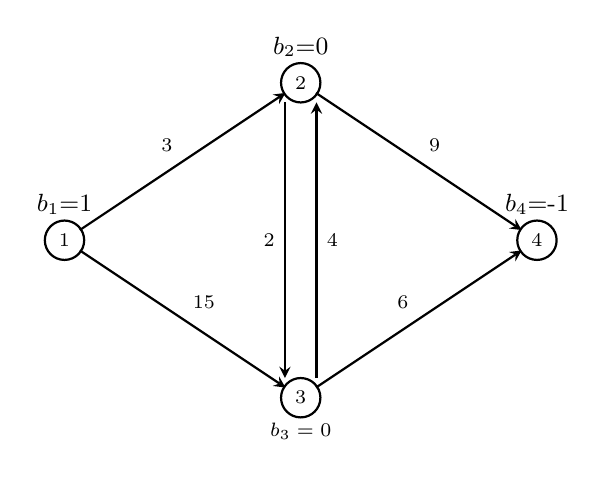
\begin{tikzpicture}
          [font=\scriptsize,
          node/.style={shape=circle,draw=black,fill=white!20, text=black,minimum width=0.5cm,thick},
          arc/.style={->,>=stealth,thick},
          edge/.style={thick}]
          
            \node (1) [node] at (0,0) {};
            \node (2) [node] at (3,2) {};
            \node (3) [node] at (3,-2) {};
            \node (4) [node] at (6,0) {};
            \node[label={\small $b_1$=1}] (1) at (0,0) {1};
            \node[label={\small $b_2$=0}] (2) at (3,2) {2};
            \node (3) at (3,-2) [label=below:{$b_3=0$}]{3};
            \node[label={\small $b_4$=-1}] (4) at (6,0) {4};
 
          \coordinate (A2) at (2.8,1.75);
          \coordinate (A3) at (2.8,-1.75);
          \coordinate (B2) at (3.2,1.75);
          \coordinate (B3) at (3.2,-1.75);
          
          \draw [arc] (1) to node [auto] {3} (2);
            \draw [arc] (1) to node [auto] {15} (3);
            \draw [arc] (A2) to node [left] {2} (A3);
            \draw [arc] (B3) to node [right] {4} (B2);
            \draw [arc] (2) to node [auto] {9} (4);
            \draw [arc] (3) to node [auto] {6} (4);

        \end{tikzpicture}
\end{center}



\noindent\underline{Indices}
\begin{tabbing}
\hspace{.5cm} \= $i\in N$ \hspace{2.5cm} \= nodes, $N=\{1,2,3,4\}$ \\
\> $(i,j)\in A$ \>  arcs \\

\noindent\underline{Data}\\% [units]\\
\> {\it c}$_{ij}$ \> cost to flow one unit (defined on figure above) \\

\noindent\underline{Decision Variables}\\% [units]\\
\> {\it X}$_{ij}$ \> Amount of flow on arc $(i,j)$  \\
\end{tabbing}

\begin{parts}
\pts{6}
We  place one unit of supply at node 1, 1 unit of demand at node 4 and zero units of supply at all other nodes. Formulate an objective function to compute the minimum cost network flow. 

 \[
    \begin{array}{llll}
      \displaystyle\min_{ \tiny{\it X}} &  3 X_{12} + 15 X_{13} + 2 X_{23} + 4 X_{32} + 9 X_{24} + 6 X_{34} & &  \\
    \end{array}
    \]

or

 \[
    \begin{array}{llll}
      \displaystyle\min_{ \tiny{\it X}} &  \sum\limits_{(i,j) \in A} c_{ij} X_{ij} & &  \\
    \end{array}
    \]

\vfill

\pts{4} Label all four nodes in the network diagram above with their ``net supply'' or $b_i$ value.

\vspace{0.5cm}

See the labels on the figure above.  Note that there is one unit of supply at node 1, one unit of demand at node 4, and nodes 2 and 3 are transshipment nodes.

\pts{6} Write the balance of flow constraint for node 3.

 \[
    \begin{array}{llll}

& X_{32} + X_{34} - X_{13} - X_{23} = 0 & & {\rm (BOF, Node~3)}\\
    \end{array}
    \]

\vfill

\pts{4} Find the optimal objective value by inspection, and write the corresponding values of the decision variables for this solution.

An optimal solution to the model shown is $X_{12}=X_{23}=X_{34}=1, ~ X_{13}=X_{32}=X_{24} = 0$, which gives an optimal objective value of 11.
\vfill

\end{parts}
\newpage

\ques{20}
US NorthWest plans to install fiber in a metro area network that is expected to experience increased demand due to the opening of a large manufacturing facility.  The Central Offices (COs) in the network are represented by vertices in the graph below.  The edges in the graph represent the possible fiber paths linking the COs.  The number on edge $(i,j)$ represents the cost $c_{ij}$ (in \$1000) of installing fiber between COs $i$ and $j$.

\begin{center}
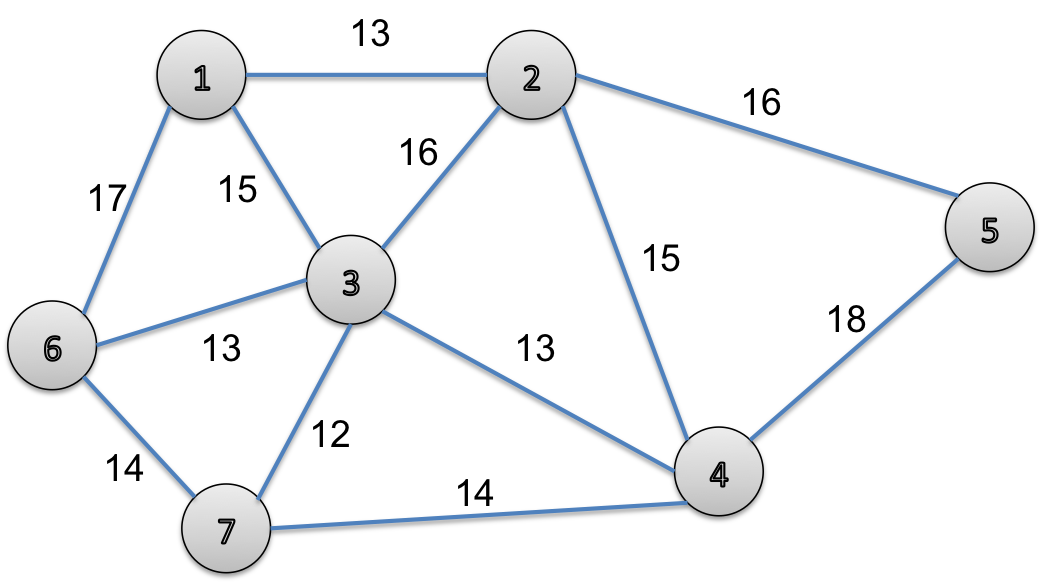
\includegraphics[width = .5\textwidth]{uswest_network}
\end{center}

Network planners developed the following integer program to solve for the collection of edges that will minimize the cost of connecting all the central offices in the network via a fiber spanning tree.  (Let $V$ represent the set of vertices in the graph.  Let $E$ represent the set of edges in the graph.)

\begin{equation}
  \label{eq:mst}
  \tag{MST}
  \begin{array}{llll}
    \min & \Sum_{(i,j)\in E} c_{ij} X_{ij} & & \\
    \mbox{s.t.} & \Sum_{j:(i,j) \in E} X_{ij} + 
    \Sum_{j:(j,i) \in E} X_{ji} \geq 1, & \forall i \in V &
    \mbox{(a)} \\[4mm]
    & \Sum_{(i,j) \in E} X_{ij} = ~? & & \mbox{(b)} \\[4mm]
    & \Sum_{\substack{i,j \in V' \\ (i,j) \in E}} X_{ij} \leq |V'| - 1 & \forall V' \subseteq V & \mbox{(c)} \\[4mm]
    & X_{ij} \in \{0,1\} & \forall (i,j) \in E. &
  \end{array}
\end{equation}



\begin{parts}
  
\pts{4} Write down the constraint of type (a) from \eqref{eq:mst} for vertex 4.

\[  \Sum_{j:(4,j) \in E} X_{4j} +  \Sum_{j:(j,4) \in E} X_{j4} \ge 1 \]
or
\[ X_{45} + X_{47} + X_{24} + X_{23} \ge 1 \]

This constraint ensures that vertex 4 is connected to at least one other node.
\vfill

\pts{2} What GUSEK code would implement the objective function? Assume that $c$, $X$ and $E$ have already been defined for you.  

\begin{verbatim}
minimize obj:sum{(i,j) in E} c[i,j] * X[i,j];
\end{verbatim}
\vfill

\newpage

\pts{6} Architect Ima Klutz spilled cappuccino on the formulation rendering the right hand side of constraint (b) illegible.  What is the purpose of constraint (b), and what should the missing number be?

\[  \Sum_{(i,j) \in E} X_{ij} = n-1 = 6 \]

The purpose of this constraint is to ensure we have $n-1$ edges in our tree that contains $n$ nodes.
\vfill

\pts{4} The modeling team learns that city ordinances require that if link $(3,7)$ is built, then neither $(1,2)$ nor $(3,4)$ may be built.  Write a constraint to model this new requirement.

\[ 2 - 2 X_{37} \ge X_{12} + X_{34} \]


We can derive this constraint from the rule that says that when we want to model the constraint ``(binary variable) $Y = 1$ implies $f \leq 0$'' we use  $f \leq M(1-Y)$ where $M$ is a constant chosen so that $f \leq M$ always holds. Here the variable $X_{37}$ plays the role of $Y$ and requiring that $X_{12} = 0$ and $X_{34}=0$ is the same as requiring that $X_{12}+X_{34} \leq 0$, so $X_{12}+X_{34}$ plays the role of $f$. The quantity $f$ is clearly always less than 2 so we can take $M = 2$. This gives the answer above. 

\vfill

\pts{4} The Central Office represented by vertex 3 is centrally located, but the equipment there is outdated.  If vertex 3 is used as a hub, meaning three or more fiber paths meet at vertex 3, the Central Office there will require a \$25,000 upgrade.  The modeling team adds a new binary variable $Y$ that indicates whether or not vertex 3 is used as a hub in the network design.  They modify the objective function by adding the term $25*Y$.  Write a constraint that forces $Y$ to be 1 if three or more selected edges connect to vertex 3.

\[ X_{13} + X_{23} + X_{34} + X_{36} + X_{37} \le 3 Y + 2 \]

We obtain this solution as follows. First we see that we want to impose the condition ``$X_{13} + X_{23} + X_{34} + X_{36} + X_{37} \geq 3$ implies $Y=1$''. This is logically equivalent to the condition that $Y = 0$ implies that $X_{13} + X_{23} + X_{34} + X_{36} + X_{37} \leq 2$. We'd like to use the rule mentioned in part (d) but our assumption is that $Y=0$, not $Y=1$. To fix this we introduce the variable $Z = 1-Y$. Now $Y=0$ precisely when $Z=1$, so we are trying to model ``$Z=1$ implies $X_{13} + X_{23} + X_{34} + X_{36} + X_{37} -2 \leq 0$''. This can be done using the rule with $f = X_{13} + X_{23} + X_{34} + X_{36} + X_{37} -2$ and $M = 3.$ We get 
\[ X_{13} + X_{23} + X_{34} + X_{36} + X_{37} -2 \leq 3(1-Z), \]
and substituting $Z = 1-Y$ we get 
\[ X_{13} + X_{23} + X_{34} + X_{36} + X_{37} -2 \leq 3Y, \]
which is equivalent to the condition that we gave as the answer above. 

\vfill

\end{parts}

% \newpage

% %%true/false/multiple choice
% \ques{10} True or False. No justification needed.
% \begin{itemize}
%   \tfl If the simplex method returns an optimal solution for a linear
%   program in canonical form with $m$ constraints and $n$ variables,
%   then the solution could have more than $n-m$ variables set to zero.

%   \tfl All feasible linear programs that are not unbounded have extreme point optimal solutions.

%   \tfl A d
% \end{itemize}
%%LP questions 20-30%




\newpage

%%some graph problems?

%%bonus question

%\bques{10}
%Recall that an undirected graph, $\cG = (\cV,\cE)$, is a tree if $\cG$ is connected (there is a path between every pair of nodes), and has no cycles. A leaf is a node in a tree with exactly one arc adjacent to it. Prove that any tree has at least two leaves, assuming that the number of nodes, $n$, is greater than or equal to two. 

% Start a path at an arbitrary node, walking to any neighbor that hasn't been visited before.  After at most $n$ steps, we must reach a node $v$ where there are no untraversed neighbors.  Therefore, $v$ must have only one neighbor and is a leaf, otherwise there is a cycle and the graph is not a tree.  We can then traverse a path starting at $v$, and the node where the path stops must be a second leaf.